% This is "sig-alternate.tex" V2.0 May 2012 This file should be compiled with
% V2.5 of "sig-alternate.cls" May 2012
%
% This example file demonstrates the use of the 'sig-alternate.cls' V2.5
% LaTeX2e document class file. It is for those submitting articles to ACM
% Conference Proceedings WHO DO NOT WISH TO STRICTLY ADHERE TO THE SIGS
% (PUBS-BOARD-ENDORSED) STYLE.  The 'sig-alternate.cls' file will produce a
% similar-looking, albeit, 'tighter' paper resulting in, invariably, fewer
% pages.
%
% ----------------------------------------------------------------------------------------------------------------
% This .tex file (and associated .cls V2.5) produces: 1) The Permission
% Statement 2) The Conference (location) Info information 3) The Copyright
% Line with ACM data 4) NO page numbers
%
% as against the acm_proc_article-sp.cls file which DOES NOT produce 1) thru'
% 3) above.
%
% Using 'sig-alternate.cls' you have control, however, from within the source
% .tex file, over both the CopyrightYear (defaulted to 200X) and the ACM
% Copyright Data (defaulted to X-XXXXX-XX-X/XX/XX).  e.g.
% \CopyrightYear{2007} will cause 2007 to appear in the copyright line.
% \crdata{0-12345-67-8/90/12} will cause 0-12345-67-8/90/12 to appear in the
% copyright line.
%
% ---------------------------------------------------------------------------------------------------------------
% This .tex source is an example which *does* use the .bib file (from which
% the .bbl file % is produced).  REMEMBER HOWEVER: After having produced the
% .bbl file, and prior to final submission, you *NEED* to 'insert' your .bbl
% file into your source .tex file so as to provide ONE 'self-contained' source
% file.
%
% ================= IF YOU HAVE QUESTIONS ======================= Questions
% regarding the SIGS styles, SIGS policies and procedures, Conferences etc.
% should be sent to Adrienne Griscti (griscti@acm.org)
%
% Technical questions _only_ to Gerald Murray (murray@hq.acm.org)
% ===============================================================
%
% For tracking purposes - this is V2.0 - May 2012

\documentclass{sig-alternate} 
\usepackage{url} 
\usepackage{color}
% \documentclass[10pt]{article} \usepackage{url} \usepackage{color}
\usepackage[utf8]{inputenc}
% \usepackage[margin=1in]{geometry}
\usepackage{amssymb}
\usepackage{amsmath}
\usepackage[inline]{enumitem}
\usepackage{amsfonts}
\usepackage[]{algorithm2e}
\usepackage{cleveref}
\crefname{section}{§}{§§}
\Crefname{section}{§}{§§}
\usepackage{graphicx}
\usepackage{authblk}
\newcommand{\fdadd}[1]{\textcolor{red}{#1}}
\newcommand{\fdcomment}[1]{\textbf{\textcolor{red}{[FD: #1]}}}
\newcommand{\ckcomment}[1]{\textbf{\textcolor{blue}{[CK: #1]}}}
\newcommand{\kmcomment}[1]{\textbf{\textcolor{green}{[KM: #1]}}}
\DeclareMathOperator{\corpus}{\mathcal{C}}
\DeclareMathOperator{\doc}{\mathnormal{d}}
\DeclareMathOperator{\sent}{\mathnormal{s}}
\DeclareMathOperator{\order}{\pi}
\DeclareMathOperator{\dtime}{\mathnormal{t}}
\DeclareMathOperator{\hour}{\mathnormal{h}}
\DeclareMathOperator{\hours}{\mathcal{H}}
\DeclareMathOperator{\Sim}{\mathbf{K}}
\DeclareMathOperator{\SMat}{\mathbf{X}}
\DeclareMathOperator{\Pref}{\boldsymbol{\pi}}
\DeclareMathOperator{\Exemp}{\mathnormal{Exemplars}}
\DeclareMathOperator{\Updates}{\mathnormal{Updates}}


\newcommand{\query}[0]{q}
\newcommand{\stime}[0]{t_s}
\newcommand{\etime}[0]{t_e}


\begin{document}

%
% --- Author Metadata here ---
%\conferenceinfo{WOODSTOCK}{'97 El Paso, Texas USA}
%\CopyrightYear{2007} % Allows default copyright year (20XX) to be over-ridden
%- IF NEED BE.  \crdata{0-12345-67-8/90/01}  % Allows default copyright data
%(0-89791-88-6/97/05) to be over-ridden - IF NEED BE.  --- End of Author
%Metadata ---

\title{The Anatomy of a Temporal Summarization System}

\numberofauthors{1} %  in this sample file, there are a *total*
\author{}
% \author[1]{Chris Kedzie}
% \author[1]{Kathleen McKeown}
% \author[2]{Fernando Diaz}
% \affil[1]{Columbia University, Department of Computer Science}
% \affil[2]{Microsoft Research}
%    Alternate {\ttlit ACM} SIG Proceedings Paper in LaTeX
%Format\titlenote{(Produces the permission block, and copyright information).
%For use with SIG-ALTERNATE.CLS. Supported by ACM.}} \subtitle{[Extended
%Abstract] \titlenote{A full version of this paper is available as
%\textit{Author's Guide to Preparing ACM SIG Proceedings Using
%\LaTeX$2_\epsilon$\ and BibTeX} at \texttt{www.acm.org/eaddress.htm}}}
%
% You need the command \numberofauthors to handle the 'placement and
% alignment' of the authors beneath the title.
%
% For aesthetic reasons, we recommend 'three authors at a time' i.e. three
% 'name/affiliation blocks' be placed beneath the title.
%
% NOTE: You are NOT restricted in how many 'rows' of "name/affiliations" may
% appear. We just ask that you restrict the number of 'columns' to three.
%
% Because of the available 'opening page real-estate' we ask you to refrain
% from putting more than six authors (two rows with three columns) beneath the
% article title.  More than six makes the first-page appear very cluttered
% indeed.
%
% Use the \alignauthor commands to handle the names and affiliations for an
% 'aesthetic maximum' of six authors.  Add names, affiliations, addresses for
% the seventh etc. author(s) as the argument for the \additionalauthors
% command.  These 'additional authors' will be output/set for you without
% further effort on your part as the last section in the body of your article
% BEFORE References or any Appendices.

%\numberofauthors{3} %  in this sample file, there are a *total*
% of EIGHT authors. SIX appear on the 'first-page' (for formatting reasons)
% and the remaining two appear in the \additionalauthors section.
%
%\author{
% You can go ahead and credit any number of authors here, e.g. one 'row of
% three' or two rows (consisting of one row of three and a second row of one,
% two or three).
%
% The command \alignauthor (no curly braces needed) should precede each author
% name, affiliation/snail-mail address and e-mail address. Additionally, tag
% each line of affiliation/address with \affaddr, and tag the e-mail address
% with \email.
%
% 1st. author

%\alignauthor Chris Kedzie\\ \affaddr{Columbia University}\\
%\affaddr{Department of Computer Science} \email{kedzie@cs.columbia.edu}

% 2nd. author
%\alignauthor Kathleen McKeown\\ \affaddr{Columbia University}\\
%\affaddr{Department of Computer Science}\\ \email{kathy@cs.columbia.edu}

% 3rd. author
%\alignauthor Fernando Diaz\\ \affaddr{Microsoft Research}\\
%\email{fdiaz@microsoft.com}

% There's nothing stopping you putting the seventh, eighth, etc.  author on
% the opening page (as the 'third row') but we ask, for aesthetic reasons that
% you place these 'additional authors' in the \additional authors block, viz.
%} 
\date{29 October 2014}
% Just remember to make sure that the TOTAL number of authors is the number
% that will appear on the first page PLUS the number that will appear in the
% \additionalauthors section.

\maketitle \begin{abstract} 
During crises such as natural disasters or other human tragedies, information needs of both civilians and responders often require urgent, specialized treatment.  Slow or ineffective information access can significantly impact the safety and health of individuals.  Monitoring and summarizing a text stream during such an event remains a difficult problem.  The temporal summarization task refers to extracting short, sentence-length updates about a seed event from a stream of text data.  We present a system which makes substantial improvements over the state of the art in temporal summarization.  Our approach predicts the salience of sentences with respect to an event and then uses these predictions to directly bias a clustering algorithm for sentence selection, increasing the novelty of the updates. We use novel, disaster-specific features for salience prediction, including geo-locations and language models representing the language typically used to describe different disaster types. 
We evaluate our system on a standard set of retrospective events using a combination of human judgements and automatic evaluation measures. We demonstrate the effect of different feature groups, and the importance of salience prediction for update precision.


\end{abstract}

% A category with the (minimum) three required fields
%\category{H.4}{Information Systems Applications}{Miscellaneous}
%A category including the fourth, optional field follows...
%\category{D.2.8}{Software Engineering}{Metrics}[complexity measures,
%performance measures]

%\terms{Summarization}

%\keywords{Extractive Summarization, Affinity Propagation}

\fdcomment{We should try to pull out as much of the TREC-specific language as possible (e.g. `run submissions', `participation in the TS track') to make the results more general.}
\section{Introduction}
\label{sec:introduction}
During crises, information is critical for first responders and those caught
in the event.  When the event is significant, as in the case of Hurricane
Sandy, the amount of information produced by traditional news outlets,
government agencies, relief organizations, and social media can vastly
overwhelm those trying to monitor the situation. Methods for identifying,
tracking, and summarizing events from text based input have been explored
extensively
%KM - I think we should consider adding other event summarizers. 
(e.g.,
\cite{allan1998topic,Filatova&Hatzivassiloglou.04a,Wang&al.11}). However,
these experiments were not developed to handle streaming data from  the large and heterogeneous
environment of the modern web. Neither were they developed to address the
information needs that arise during  crisis
situations. 
%KM - this last sentence sounds somewhat negative.
%there is still a need for robust and scalable 
%methods for automatic summarization.

In this paper, we present an update summarization system to track disasters
across time. Our system predicts sentence salience in the context of a
large-scale event, such as a disaster,  and integrates these predictions into
a clustering based multi-document summarization system. We train a regression
model to predict sentence salience and use these predictions to bias the
formation of sentence clusters around more salient regions in the input space
using affinity propagation (AP) clustering.  AP uses the salience predictions
as well as pairwise similarities among input sentences to identify
\emph{exemplar} sentences, which we use as our summary output.  Our approach
differs from other methods of summarization that compute salience by pairwise
comparisons alone, ignoring features of importance that are intrinsic to the
sentences themselves.

%KM - Chris - add a short overview on the kinds of things we measure and
%results so people are encouraged to read ahead. Keep it general.

In addition to the tight integration between clustering and salience
prediction, our approach also exploits knowledge about disaster to determine
salience. Thus, salience does not just represent importance within a set of
documents; it also represents both how typical this sentence is of the input event
type (i.e., disaster, hurricane, tornado) and whether it specifies information
about this particular disaster. We use a set of language models, one for each
disaster type, to measure typicality of the sentence for the current event type. We
use a feature that measures distance of mentioned location from the center of
the disaster to represent its likelihood of referring to the input disaster. 




%Previous work on generating event descriptions and/or multi-document
%summarization has relied on clustering algorithms to find representative
%sentences appropriate for an event summary.  These methods impose a metric
%space on the text data that can make it difficult to incorporate external
%sources of information elegantly -- in this paper we argue that centroid
%sentences are not a priori the best candidates for inclusion in an event
%summary.



The remainder of the paper is organized as follows. We begin with a review of related work in the information retrieval and multi-document summarization literature.  In section
~\ref{sec:background} we give an overview of the semantic similarity,
%KM - Chris can you update this so it reflects the contributions. We don't
%mention semantic similarity. We do mention salience and the disaster specific
%features. Perhaps we should mention the use of a new approach for semantic
%similarity? 
Gaussian process, and affinity propagation algorithms that make up the bulk of
our TS system. 
Next we describe the data with which we build our various models.
Then in section~\ref{sec:approach} we give a high level sketch
of our system, and then explain each component in detail. 


\section{Related Work}
\label{sec:relatedwork}
A principal concern in extractive multi-document summarization is the
selection of salient sentences for inclusion in summary output
\cite{nenkova2012survey}.  This has often been approached as a ranking
problem.
%We broadly conceptualize this decision as either an intrinsic or extrinsic
%sentence evaluation process. Intrinsic approaches evaluate sentences
%individually, possibly by predicting the impact on summary quality using
%sentece level features. 
Sentences have been ranked by the average word probability, average tf-idf
score, and the number of topically related words (topic-signatures in the
summarization literature)
\cite{nenkova2005impact,hovy1998automated,lin2000automated}. The first two
statistics are easily computable from the input sentences, while the third
only requires an additional, generic background corpus.  Another ranking
approach, centroid summarization, involves creating an average bag of words
(BOW) vector, the centroid, from the input sentences and ranking sentences by
their similarity to the centroid \cite{radev2004centroid}.  Graph
\cite{erkan2004lexrank} and clustering
\cite{hatzivassiloglou2001simfinder,mckeown1999towards,siddharthan2004syntactic}
based approaches, on the other hand, make use of pair-wise similarity
comparisons amongst input sentences.  In these models, salient sentences are
more central to the input or cluster, respectively.

%identify salient regions of the input space while simultaneously coping with
%redundancy.  Graph-based algorithms have been used to rank sentences
%Clustering algorithms, e.g., are commonly used to exploit redundancy in
%input. Input sentences are clustered and summaries are generated by selecting
%the most representative sentence from each cluster.  Graph-based models have
%also been used for summarization.  E.g., the LexRank algorithm treats
%sentences as nodes in a graph, where edges are constructed by way of cosine
%similarity between sentence nodes; edges are either continuosly weighted by
%similarity or discrete, existing only when the similarity is above a
%threshold.  The PageRank algorithm is used on the graph to find the most
%important sentence nodes. In both clustering and graph-based approaches,
%sentence salience is largely determined by the pairwise relations between
%sentences.

Supervised learning has also been applied to this task. Model features are
usually derived from human generated summaries, and are non-lexical in nature
(e.g., sentence starting position, number of topic-signatures, number of
unique words, word frequencies). Seminal work in this area has employed naive
Bayes and logistic regression classifiers to identify sentences for summary
inclusion \cite{kupiec1995trainable,conroy2001using}. 

%\fdadd{
Several researchers have recognized the importance of summarization during
natural disasters.  Guo \textit{et al.} developed a system for detecting
novel, relevant, and comprehensive sentences immediately after a natural
disaster \cite{qi:temporal-summarization}.  The method uses a model of
sentence relevance and novelty in order to select appropriate updates.
Training data for regression targets is automatically generated from
retrospective Wikipedia data.  The system is evaluated on news documents
related to 197 natural and human disasters from 2009 to 2011 using variants of
Rouge modified to capture novelty, relevance, and comprehensiveness
\cite{lin2004rouge}.  Wang and Li present a clustering-based approach to
efficiency detect important updates during natural disasters
\cite{wang:update-summarization}.  The algorithm works by hierarchically
clustering sentences online, allowing the system to output a more expressive
narrative structure than Guo \textit{et al.}.  The method is evaluated on
official press releases related to Hurricane Wilma  in 2005 using Rouge score
between the system summary and a manually generated target summary.


\section{Motivation}

%KM If we are short on space, not sure how much this section is needed as it's
%somewhat repetitive of intro.

%KM - Chris, could you get some good references to work in the crisis
%informatics space.
Crisis informatics\cite{?} is dedicated to finding methods for sharing the
right information in a timely fashion with relief organizations during a major crisis. With the
increasing impact of climate change, the world is seeing an increase in
disasters such as hurricanes, tornadoes, flooding and typhoons, all of which
cause major damage and wreak havoc with food supplies, housing, and health
issues. Health epidemics, such as the ebola crisis in West Africa, also create
a need for timely information about where problems are greatest. Social and
political 
crises, such as the current situation in Syria, create similar needs for
humanitarian assistance.

At times of crisis, however, social media can overwhelm current information
systems with the quantity of information, much of which is irrelevant,
unnecessary detail, or out of date. Many approaches have focused on
human-in-the-loop approaches \cite{?} to enable people on the ground to update
crisis interfaces with information about needs. Others have ..
%KM - Chris - fill this out a bit.





%KM - PRobably should make a little more inclusive, there are graph based
%models that use methods such lexical similarity to build the graph,
%probabilistic methods (e.g., based on word probabilities, regression or
%topical signatures). There are also methods that use topic segmentation or
%modeling and select sentences for each topic.



Multi-document summarization offers potential for enabling automatic updates of
relevant, salient information at regular intervals. It would provide
information even when human volunteers are unable to and would filter out
unnecessary and irrelevant detail. 
Most generic multi-document summarization approaches involve either sentence 
clustering or ranking sentences according to metrics that measure the salience
of their words. 
When the summarization task
is broad or underspecified,
%clustering is most appropriate in that the data
these methods are appropriate as they let the data
``to speak for itself.''
%This is probably most true when summarization is 
%interpreted to mean exploratory data analysis. 
When there are more constraints on the output, as in query-focused
summarization or the crisis update task we present here,
results are more accurate when
%often easier to design
appropriate features for the ranking approach are used (e.g., amount of word
overlap for the query-focused approach).
%either by rule or learning-to-rank.
The primary contribution of this paper
is a framework for combining both of these approaches using affinity
propagation clustering as well as disaster-specific features.


\ckcomment{Not sure how to present this together, we also essentially evaluate
a salience model by feature ablation for the TS task, but this feels very specific compared to the general framework idea.}

\fdcomment{I guess I think we need to two things in this section (and/or introduction).  1. explain why the problem matters.  2. explain why our approach is compelling.  }

\fdcomment{if easy to generate, would be good to have a single figure for an event that includes 1. the query, 2. the distribution of (filtered) document volume over time, and 3. a sample of the gold nuggets.  this provides the reader with a visual explanation of the problem, the solution, and the difficulty}


\section{Problem Definition}
\label{sec:problemdefinition}
In order to evaluate a temporal summarization system, we adopt the simulation-based approach used in the TREC Temporal Summarization Track.  We provide a brief overview of the problem.  Details on the formulation can be found in the track overview paper \cite{aslam2013trec}.  

A temporal summarization system takes as input 
\begin{enumerate*}[label=\itshape\alph*\upshape)]
  \item a short query $\query$ defining the event to be tracked (e.g. `Hurricane Sandy'), 
  \item an event category $\eventcategory$ defining the type of event to be tracked (e.g. `hurricane'), 
  \item a stream of time-stamped documents, $(\doc_0, \doc_1,\ldots,\doc_T)$, presented in temporal order, and
        \item an evaluation time period of interest, $(\stime,\etime)$.  
\end{enumerate*}
While processing documents throughout the time period of interest, the system
must output sentences, known as updates, which are \emph{relevant} to the
query, \emph{comprehensive} with respect to the event, \emph{novel} to the
user, and \emph{timely} with respect to when the update occurred.  Precisely
how to measure these properties will be discussed in Section \ref{sec:methods}.
In our version of this problem, we assume that that the system receives one
batch of new sentence-segmented documents every hour throughout the period of
interest.

We address  disaster types such as terrorism and mass shootings (e.g.,
the 2012 shooting in Aurora, Col.), natural disasters (e.g., Hurricane Sandy),
accidents (e.g., the 2012 Pakistan garment factory fire), astronomical
disasters (e.g,. the Chelyabinsk comet in Russia), and social activism (e.g.,
the Arab spring).
\kmcomment{This was as best as I could do on this. These are the example
  categories from the wikipedia page. However you refer in the language model
  description to the event type earthquake which is more specific. Also, in the
  TREC data you refer to event types that are specified in the metadata. So I'm
  wondering how many different categories you have and where they come from.}

\fdcomment{include description of nuggets here.}
\kmcomment{We should jointly discuss what goes in data and what goes in problem
  definition. I have moved event types here because I think knowing how many
  types and examples of them would be helpful upfront. I think where nuggets
  and wikipedia pages go is questionable.}


\section{Algorithm}
\label{sec:background}

Figure \ref{alg:temporal-summarization} outlines our general temporal summarization algorithm.  At each hour, the system processes each document in the batch. It first discards any documents below a predefined relevance threshold (Section \ref{sec:filtering:documents}).  It then discards any sentences from the remaining documents which are unlikely to carry content (Section \ref{sec:filtering:sentences}).  Following this filtering process, the system must decide which of the remaining sentences should be considered an update.  We refer to this as salience prediction and describe a feature-based model for predicting salience (Section \ref{subsec:Predict}).  Because a single sub-event may produce several high-quality-but-redundant sentences within an hour, we employ a cluster-based method for selecting exemplars of high salience sub-events (Section \ref{sec:ap}).  Finally, we employ a final deduplication phase to ensure that we only select novel updates (Section \ref{sec:novelty}).

% \begin{figure}
% \centering 
\begin{algorithm}%[H]
 \KwData{\\$Query$ --- the set of event query words\\ 
        $SC$ --- the stream corpus\\

         
}
 ~\\
 Initialize empty list $\mathbf{U}$ of updates\\
 Initialize empty list $\boldsymbol{\Pref}^{(U)}$ of update preferences\\
 $\corpus \gets \operatorname{FilterDocuments}(Query, SC)$ (See \cref{sec:filtering:documents})\\
 \For{$i \gets 1,\ldots,t $}{

  Initialize empty lists $\SMat, \Pref$ \;
      

  \For{$\doc \in \corpus_{\hour_i}$}{
   \For{$\sent \in \operatorname{FilterSentences}(\doc, Query)$ (See \cref{sec:filtering:sentences})\\}{
     $\SMat.\operatorname{append}(\sent)$\;
     $\sigma \gets \operatorname{PredictSalience}(\sent)$ (See \cref{subsec:Predict})\\     
     $\Pref.\operatorname{append}(\sigma)$\;
     
   }        
  }
  %$\Sim \gets \operatorname{ComputeSimilarityMatrix}(X)$\;
  %$\operatorname{}$
  ~\\ 
  $\mathbf{U}_{h_i}, \Pref^{(U)}_{h_i} \gets \operatorname{SentenceSelection}
    (\SMat, \Pref)$ (See \cref{sec:ap})\\
  ~\\
  $\operatorname{Emit}(\mathbf{U}_{h_i})$ \\ 
  $\mathbf{U}\operatorname{.append}(\mathbf{U}_{h_i})$ \\
  $\mathbf{\Pref}^{(U)}\operatorname{.append}(\Pref^{(U)}_{h_i})$ \\
%gets \Updates_{cache} \cup \Updates_{\hour}$\;

 } 
 \caption{Temporal Summarization Algorithm}\label{alg:temporal-summarization}
\end{algorithm}
% \end{figure}

\subsection{Filtering Content}
\label{sec:filtering}
We simulate our system using realistic data insofar as the document stream consists of relevant and non-relevant content.  As with many information retrieval systems, we use a crude, first phase of high-recall content filtering for both documents and sentences.  

\subsubsection{Filtering Documents}
\label{sec:filtering:documents}
As a first filter, we retained only those documents whose raw html content contains at least one keyword from the event's query words. We further restricted our document set to only those articles from the news domain.\footnote{This filtered set was distributed by track organizers.} \fdcomment{not sure how much we have to describe this.}

\subsubsection{Filtering Sentences}
\label{sec:filtering:sentences}
Structural html artifacts and sentence tokenization errors can negatively effect the performance of a temporal summarization system. Examples of the former include strings of link text like ``World Politics Sports ...'', while examples of the latter included concatenations of unrelated content  (e.g. segmentation errors treating two headlines as a single sentence).  


In order to filter out these problematic inputs, we trained a classifier to identify which sentences came from inside a document's main article and which came from various headers, titles, menus, and links to other content. We collected random sentences and manually labeled whether the sentence came from inside or outside the document's main article. We then trained a logistic  regression classifier using: 
\begin{enumerate*}[label=\itshape\alph*\upshape)]
	\item the position of the sentence,
	\item word counts,
	\item the last token in the sentence,
	\item the last two tokens in the sentence, and
	\item the last three tokens in the sentence.
\end{enumerate*}
These features were sufficient to capture the main difference between content and non-content sentences, which  was that content sentences generally ended with sentence final punctuation, i.e. periods or a closing quotation mark. \fdcomment{include summary performance numbers here; also a reference to prior work.}

After identifying the subset of a document's sentences that are content sentences, we check to make sure \emph{all} event query terms can be found within the document's content sentences. If so, we send the content sentences on to the next stage of our pipeline; otherwise we ignore all sentences in this document.


\subsection{Predicting Sentence Salience}
\label{subsec:Predict}
Once the input has been filtered down to a higher quality set of candidate updates, we can rank sentences according to their salience.  We adopt a model-based approach to predicting salience: a good model should predict higher values for sentences that are more likely to appear in a human generated summary of the event.   The response variable we try to predict is a sentence's semantic similarity \cite{guo:wtmf} to the gold nugget sentences, i.e. we want to predict the similarity to a gold nugget when the gold nugget is not known.  If sentence is very similar to a nugget, then it is a better candidate for emission as an update compared to a sentence that is not similar to any nuggets.


\subsubsection{Features}
We want our model to be predictive across different kinds of events so we avoid lexical features.  Instead, we extract a variety of features including language model scores, geographic relevance, and temporal relevance from each sentence.  These features are used to fit a Gaussian process regression model that can predict the similarity of a sentence to a gold summary \cite{preotiuc2013temporal}.  
\fdcomment{can we enumerate all of these?}

\paragraph{Basic Features}

We employ several basic features that have been used previously in supervised models to rank sentence salience \cite{kupiec1995trainable,conroy2001using}. These include sentence length, the number of capitalized words normalized by sentence length, document position, number of named entities.  

\paragraph{Query Features}

Query features measure the relationship between the sentence and the event query and type.  These include the number of query words present in the sentence in addition to the number of event type synonyms, hypernyms, and hyponyms as found in WordNet \cite{miller1995wordnet}.  For example, for event type \emph{earthquake},  we match sentence terms ``quake'', ``temblor'', ``seism'', and ``aftershock''.


\paragraph{Language Model Features}\label{subsubsec:lm}
Language models allow us to measure the likelihood of a sentence having been produced from a particular source.  We consider two types of language model features.  The first model is estimated from a corpus of generic news articles.  This model is intended to assess the general writing quality (grammaticality, word usage) of an input sentence and helps us to filter out text snippets which are not sentences (e.g., web page titles).  The second model is estimated from text specific to our event types.  For example, the language model for event type `earthquake' is estimated from Wikipedia pages under the category \emph{Category:Earthquakes}.  These models are intended to detect sentences similar to those appearing in summaries of other events in the same category (e.g. most earthquake summaries are likely to include higher probability for ngrams including the token `magnitude').  


%For both models, we Finally, we extract the percentage of capitalized words,
%and sentence length as features. These last two features also help to
%identify sentences that are less likely to contain relevant content-- overly
%long and heavily capitalized sentences in our corpus were likely to be long
%strings of web-page headlines, section headers, and other irrelevant page
%structure. 

\paragraph{Geographic Relevance Features}

Locations are identified using a named entity tagger. For each location in a sentence, we obtain its latitude and longitude using the a publicly available geolocation service.  We then compute its distance to that of the event location.  It is possible for a sentence and an event to have multiple locations so we take as features the minimum, maximum, and average distance of all sentence-event location pairs.  Distances are calculated using the Vincenty distance. 

\paragraph{Temporal Relevance Features}

Our data consists of hourly crawls of online content and so we exploit the temporality of corpus by capturing the burstiness of a sentence, i.e.  the change in word frequency from one hour to the next.``Bursty'' sentences often indicate new and important data. 

Let $D_t$ be the set of web pages at time $t$ and let $s = \{w_1,\ldots,w_n\}$ be a sentence from a page $d \in D_t$.  We calculate the 1-hour burstiness of sentence $s$ from document $d$ at hour $t$  as 
\begin{align*}
\operatorname{b}_1(s,d,t) = \frac{1}{|s|} \sum_{w \in s} \Bigg( &
\operatorname{tf-idf}_t(w,d)  \\ & \left. - \frac{\sum_{d^\prime \in D_{t-1}:
w \in d^\prime } \operatorname{tf-idf}_{t-1}(w,d^\prime)}{|\{d^\prime \in
D_{t-1}: w \in d^\prime\}|} \right) \end{align*}

where \begin{align*} \operatorname{tf-idf}_t(w,d) =&
\log\left(1+\sum_{w^\prime \in d}1\{w=w^\prime\}  \right)\\ & \times
\log\left(\frac{|D_t|}{1 + \sum_{d^\prime \in D_t}1\{w \in d^\prime\}}\right).
\end{align*}
% 1\{w = w^\prime} %- \operatorname{avg-tf-idf}_{t_{i-1}}(w).
%\end{align*}


We similarly find the sentence's 5-hour burstiness.  In addition to burstiness, we also include the sentence's average tf-idf and hours since the event in question started as features.

\subsubsection{Gaussian Process Regression}

\fdcomment{transition to gp description}

A Gaussian process (GP) is a distribution over functions and is a 
generalization of the multi-variate Gaussian to the infinite dimensional
setting. That is, we use the observed data to define a distribution over 
possible functions that generated this data, without having to explicitly 
parameterize the function---in this sense GPs are considered 
a non-parametric model.

Formally, let $p(f)$ be a distribution over functions where $f$ is any mapping
of an input space $\mathcal{X}$ to the reals,

$$f: \mathcal{X} \rightarrow \mathcal{R}.$$ 
Let the random variable $\mathbf{f} = (f(x_1),\ldots,f(x_n) )$ be
 an $n$-dimensional vector whose elements are evaluations of the function $f$
at points $x_i \in \mathcal{X}$.
We say $p(f)$ is a Gaussian process if for any finite subset 
$\{x_1,\ldots,x_n\} \subset \mathcal{X}$, the marginal distribution over 
that finite subset $p(\mathbf{f})$ has a multivariate Gaussian distribution.
A GP is parameterized by a mean function $\mu(\mathbf{x})$ and a 
covariance function $K(x,x^\prime)$. Generally, the mean function is simply
set to 0, leaving the distribution to be completely characterized by the
kernel function on the data.

In the regression setting, we typically have a response variable $y$ that
is the sum of our model prediction  and 
some Gaussian noise, i.e. $y = f(x) + \epsilon$ with 
$\epsilon \sim \mathcal{N}(0, \sigma^2)$. When
$f \sim \operatorname{GP}(\mathbf{0}, \mathbf{K})$, the
two distributions
of principal interest are the marginal likelihood
$p(\mathbf{y}|\mathbf{X}) = 
\mathcal{N}(\mathbf{0},\mathbf{K} + \sigma^2\mathbf{I})$ and the predictive
distribution,

$$p(\mathbf{y_*}|\mathbf{x_*},\mathbf{X},\mathbf{y}) =
\mathcal{N}(\boldsymbol{\mu}_*, \boldsymbol{\sigma}^2_*) $$

where $\mathbf{x_*}$ is a new or unseen input, $\mathbf{y_*}$ our predicted
response, and
\begin{align*}
\boldsymbol{\mu}_* & = \mathbf{K_*}(\mathbf{K} + \sigma^2\mathbf{I})^{-1}\mathbf{y} \\
\boldsymbol{\sigma}^2_* & 
= \mathbf{K}_{**} - \mathbf{K}_*(\mathbf{K} + \sigma^2\mathbf{I})^{-1}
\mathbf{K}_*^T + \sigma^2\\
\end{align*}.

Here $\mathbf{K}_* = K(\mathbf{x}_*, \mathbf{X})$, and 
$\mathbf{K}_{**} = K(\mathbf{x}_*, \mathbf{x}_*)$.


GP's are incredibly general, and are state of the art for many regression 
tasks (?). The reliance on the covariance matrix 
$\mathbf{K}$ for parameterization opens up the wide world of kernel methods
for regression, and many varieties of similarity functions can be used.
In our experiments we used a radial basis function kernel 
$$K(\mathbf{x},\mathbf{x}^\prime) = \sigma^2 \exp\bigg(- \frac{1}{2} 
\sum_{i=1}^d \frac{ (x_i-x^\prime_i)^2}{\ell_i^2} \bigg)$$ where 
$\sigma$ and the $\ell_i$ are parameters we fit to our observed training data.
The $\ell_i$ are feature dependent scaling parameters; once learned, they not
only improve the accuracy of the model, but give us some introspection 
into which features are more important.

\subsection{Selecting Sentences}
\label{sec:ap}
In the sentence selection stage, we use the salience predictions from our GP
model as preferences in the AP clustering algorithm. The AP algorithm is 
parameterized by a similarity matrix $\mathbf{S}$ and a vector of 
preferences $\boldsymbol{\pi}$; we found AP to be very sensitive to these
parameters, and did not perform robustly on our range of inputs.
In order to improve the quality of the clusters and exemplar selection,
we re-scaled both the raw inputs $\mathbf{S}$ and $\boldsymbol{\pi}$. 
The raw preferences are scaled to lie within the  range $(-3, -2)$

The initial matrix $\mathbf{S}$ is computed by finding the pairwise semantic
similarity between input sentences. Self-similarities and similarities below 
a threshold $\lambda$ were masked and the remaining values scaled to the range
$(-3, -1)$.

\subsubsection{Semantic Similarity}\label{subsec:semsim}

Whenever we make a pairwise comparison between sentences, we use the weighted
textual matrix factorization (WTMF) model of \cite{guo2012simple}. This 
model can be thought of as a variant of latent semantic analysis (?), 
where words that are not present in a sentence are explicitly modeled.
More formally, we have a term-sentence matrix 
$\mathbf{X}\in\mathcal{R}^{v \times n}$ representing $n$ sentences with a 
vocabulary of $v$ words; $\mathbf{X}_{i,j}$ indicates is non-zero if sentence
$j$ contains word $i$. In the WTMF regime, we want to find an approximation
of $\mathbf{X} \approx \mathbf{P}^T\mathbf{Q}$, where 
$\mathbf{P} \in \mathcal{R}^{k \times v}$ is a latent word vector space and
$\mathbf{Q} \in \mathcal{R}^{k \times n}$ is a latent sentence vector
space. These matrices are found by minimizing the objective function

$$\sum_i^v \sum_j^n \mathbf{W}_{i,j}(\mathbf{P}_{\cdot,i}^T
\mathbf{Q}_{\cdot,j} 
- \mathbf{X}_{i,j})^2 
 + \lambda ||\mathbf{P}||_2^2 + \lambda ||\mathbf{Q}||_2^2$$

where $\mathbf{W}_{i,j} = 
\begin{cases} 1, & \textrm{if $\mathbf{X}_{i,j} \ne 0$ } \\
w_m, & \textrm{if $\mathbf{X}_{i,j} = 0$ }\\
\end{cases}$
and $\lambda$ is a hyperparameter controlling the regularization terms.

The $w_m$ term is another model hyperparameter that is set to a small constant
($\le .01$). The weight matrix $\mathbf{W}$ has the effect of discounting the
reconstruction error of missing terms (words that did not occur a sentence).

Given an unseen sentence $\hat{i}$ we can project its term vector into the
latent sentence vector space with 

$$
\mathbf{Q}_{\cdot,\hat{i}} = (\mathbf{P}\mathbf{\tilde{W}}^{(\hat{i})}
\mathbf{P}^T  + \lambda\mathbf{I} )^{-1} 
\mathbf{P}\mathbf{\tilde{W}}^{(\hat{i})} \mathbf{X}_{\cdot, \hat{i}}
$$  

where $\mathbf{\tilde{W}}^{(\hat{i})}$ is an $v\times v$ diagonal matrix
where $\mathbf{\tilde{W}}^{(\hat{i})}_{j,j}$ is equal to $1$ or $w_m$ 
depending on whether or not the $j$-th term occurs in sentence $\hat{i}$.


The WTMF model is used extensively throughout our TS system. When making any 
pairwise comparison between sentence $i$ and $j$, we first construct
their latent sentence vectors $\mathbf{Q}_{\cdot,i}$ and
$\mathbf{Q}_{\cdot,j}$ and then find the cosine similarity 
$\displaystyle \operatorname{cos-sim}
(\mathbf{Q}_{\cdot,i}, \mathbf{Q}_{\cdot,j}) = 
\frac{\mathbf{Q}_{\cdot,i}^T\mathbf{Q}_{\cdot,j}}{||\mathbf{Q}_{\cdot,i}||_2
||\mathbf{Q}_{\cdot,j}||_2   }$.


Because the events for the TS task come from different domains, we construct
domain specific latent word vector spaces for each domain using in-domain 
Wikipedia pages (see~\cref{sec:data} for more details).


\subsubsection{Affinity Propagation}
Affinity propagation (AP) is a message passing algorithm that identifies both
exemplar data points and assignments of each point to an exemplar.  This is
done iteratively by passing \emph{responsibility} and \emph{availability}
messages between data points that quantify the fitness of one data point to
represent another, and the fitness of a data point to be represented based on
the choices of other data points respectively \cite{dueck2007non}.

AP is parameterized by an $n\times n$ similarity matrix $S$ and an $n\times 1$
preference vector $\pi$.  $S$ is a real-valued matrix where $S(i,j)$ is the
similarity of the $i$-th data point to the $j$-th data point.  $S$ does not
need to be symmetric.  $\pi$ is a real-valued vector where $\pi(i)$ expresses
our preference that the $i$-th data point can serve as an exemplar a priori of
other data points. 




AP has several useful properties that comport well with the TS track 
requirements. First, the number of clusters $k$ is not a hyper-parameter
of the model. Since we will be running this algorithm many times in per run,
the usual methods of hyperparameter search become infeasible 
(?). The number of clusters falls out of the algorithm
organically-- lower overall preference values will result in fewer clusters. 

Secondly, the arbitrary nature of the preferences
allow us to incorporate a variety of signals for
identifying the best exemplars, i.e. salience and redundancy signals. 
The preferences can be thought of as self-similarities (similarities that
pairwise-comparison based algorithms would ignore) that we can exploit to 
incorporate our prior beliefs about a data point.

Finally, cluster exemplars are guaranteed to be actual data points. Many 
clustering algorithms group data around mathematical objects (e.g., the
mean) that are not necessarily observed in the data. The extractive nature of
this TS task requires that we emit actual data points (i.e. sentences).
We are able to sidestep 
the additional requirement of selecting a most
representative cluster member, as this is computed explicitly in the AP 
algorithm. 

\subsubsection{Preferences}

Before rescaling, we first penalize each $\boldsymbol{\pi}_i$ based on
the aggregate similarity of input sentence $\mathbf{s}_i$ to the set of previous updates
$\mathbf{U}$. We call this the redundancy penalty 

$$\rho_i = \sum_j \frac{\boldsymbol{\pi}^{(U)}_{j}\operatorname{cos-sim}(\mathbf{s}_i, \mathbf{U}_j)}
{\sum_{j^\prime}\operatorname{cos-sim}(\mathbf{s}_i, \mathbf{U}_{j^\prime})} $$   
where $\boldsymbol{\pi}^{(U)}_{j}$ is the salience prediction of the $j$ 
previous update. We calculate our new penalized preferences 
$\boldsymbol{\pi}^{(\rho)}$ where $\boldsymbol{\pi}^{(\rho)}_i = \boldsymbol{\pi}_i - \rho_i$.
Finally, we rescale $\boldsymbol{\pi}^{(\rho)}$ such that all values lie 
within the range $(-3,-2)$.


\subsection{Ensuring Novelty}
\label{sec:novelty}
We run AP clustering with our rescaled and penalized sentence similarities
and preferences. When the clustering has converged we emit all exemplar
sentences (cluster centers) whose preference is $\lambda$ standard deviations
above the mean preference for the current time period and who do not belong
to singleton clusters as updates. These updates and their preferences are 
retained for penalty calculations in subsequent time steps.






\section{Methods}

\subsection{Data}\label{sec:data}

Our primary datasets are the TREC 2013/2014 Stream Corpus, 
a ?tb corpus of hourly 
web crawls from October 2011
through mid February 2013 \cite{frank2012building}.\footnote{\url{http://trec-kba.org/kba-stream-corpus-2014.shtml}}
As per the TS specifications, all summary sentences come from processing this
corpus in a time aligned manner. While the 2014 corpus encompasses the 
2013 corpus, we use the 2013 corpus for evaluating events from the 2013 track
year because sentence ID's used in evaluation changed from year to year.

For our semantic similarity component (\cref{subsec:semsim}),
domain specific term-sentence matrices were built using subsections of
Wikipedia. For each event type we identified one or more related Wikipedia
categories and collected all pages that were listed under that category.
For all pages collected, we used the latest possible revision date before the
start of the Stream Corpus.

We use the same Wikipedia corpora to construct the lanuage models used
in our salience prediction model (\cref{subsubsec:lm}). 

\begin{figure*}
	\begin{center}
\begin{tabular}{| p{5cm} c c |}
\hline
Event & WP Categories & No. Docs/Sents/Words\\
\hline \hline
Boston\_Marathon\_bombings \newline
Christopher\_Dorner\_shootings\_and\_manhunt \newline 
 In\_Amenas\_hostage\_crisis
& Terrorism, Mass Shootings & 33,732/1,139,588/26,201,659  \\
\hline
 Cyclone\_Oswald \newline
Early\_2012\_European\_cold\_wave \newline
February\_2013\_noreaster \newline & Weather events & 35,554/591,850/12,794,438  \\
\hline
Costa\_Concordia\_disaster & Accidents & 22,874/732,945/16,520,242 \\
\hline
Chelyabinsk\_meteor & Earthquakes & 14,515/283,509/6,135,803  \\
\hline
Port\_Said\_Stadium\_riot \newline
2012\_Afghanistan\_Quran\_burning\_protests \newline
2011-13\_Russian\_protests \newline
2012\_Romanian\_protests \newline
2012-13\_Egyptian\_protests \newline
2013\_Bulgarian\_protests\_against\_the\_Borisov\_cabinet \newline
2013\_Shahbag\_protests & Activism\_by\_type & 464,657/11,254,122/250,172,896  \\
\hline
\end{tabular}
\caption{Domain specific Wikipedia corpora for semantic similarity and 
language models. }
\end{center}
\end{figure*} 

\subsubsection{Events}

We use the event set developed for the TREC Temporal Summarization track 
for years 2013 and 2014. There were 10 and 15 events respectively. We omit
one event from the 2013 track because there were no news documents in the 
corpus during the duration of the event, yielding a final event set of 24 
events. Meta-data provided for each event includes the name of the event
as it appears on Wikipedia, a short text query for the event, 
the type of event, and the 
duration of the event (the duration for the system 
to monitor not necessarily the complete timespan of the event). 
All data except the Wikipedia name is exposed to the TS system to use.  

\subsubsection{Nuggets}
For evaluation purposes, important pieces of information, hereafter 
referred to as nuggets, were extracted from each event's Wikipedia page.
Assessors graded nuggets by importance, and were also able to timestamp their
existance using the timestamp of the page's revision history. Nuggets are 
usually a short to medium length clause containing an atomic piece of
information.

\subsubsection{Matches}
TREC assessors provided judgements on a subset of participant updates each year
of the track. Judged updates are matched to one or more nuggets (a real 
sentence often contains more than one atomic piece of information) or marked
not relevant. There was not much overlap in the participant update sets so
overall coverage of relevant sentences in the corpus is small (percent?).
To expand the judgement corpora, we include all system updates as positive
nugget matches if they are $< .2$ close in Levenshtein distance to a human
assessed matched update. 

\subsection{Experiment Design}

\subsubsection{Salience Models}
For each event (both in the complete system and feature ablation experiments)
we randomly sample 1000 sentences after relevant document filtering and 
over the duration of the event 
(as determined by 
TREC; avg. run length is ? days) of the event. Nugget similarities
are computed for each sentence and are standardized with respect to 
the sample mean and variance. After standardization, the maximum nugget similarities are computed for each sentence. 
We fit a Gaussian process for each event, using the maximum similarities 
as our regression target, yielding 24 models in total. Kernel lengthscale
parameters are also individually fit for each model.
When making event-specific predictions, we take the average prediction of the
23 other models.

\subsubsection{Redundancy Threshold}

For every time interval with input, a clustering algorithm is
guarranteed to produce at least one output; 
this can significantly hurt the performance of all clustering based 
temporal summarization systems. In order to avoid this, we set a threshold $t$
such that a new update must have a maximum similarity $< t$ to all previous 
updates.

We determined the value of $t$ by examining the distribution of similarities
of nuggets to their human-matched sentences compared to the distribution
of similarities of nuggets to relevant but non matching sentences. We fit
normal distributions for the matching and non-matching similarities and
used the point of intersection as the value of $t$.
Figure ? shows a normalized histogram of cosine similarities for both 
distributions, the fitted distributions, and the point of intersection.

\begin{figure}
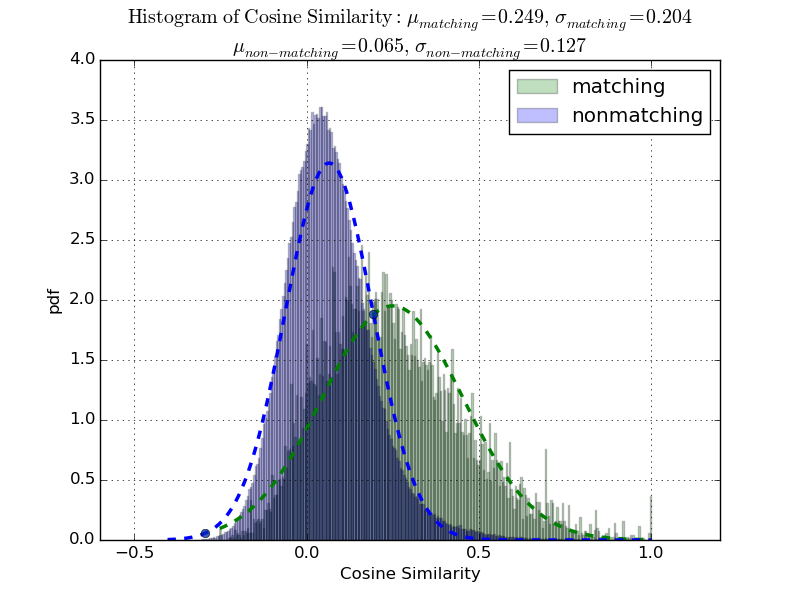
\includegraphics[scale=.40]{match-dist.png} 
\caption{Distribution of nugget similarity for matching and non-matching 
updates.}
\end{figure}
\subsubsection{Effect of Salience Models}

In order to assess the effectiveness of the salience predictions on update
selection, we perform a baseline (AP-base) run using affinity propagation 
clustering
with uniform preference, i.e. all preferences are equal to the median sentence
similarity. This run is compared to our full system (AP-sal), using each
sentence's salience prediction as its preference. 

We are also interested
in the effect of directly incorporating salience in the clustering algorithm.
A third run (HAC) is performed using hierarchical agglomerative 
clustering; we produce flattened clusters by setting a maximum cluster 
distance threshold. The sentence with the highest predicted salience from each
 cluster is selected as an update. 
The distance threshold was tuned using grid search. By comparing
HAV with AP-base we can empirically assess the trade off between preference
and neighbor similarity that affinity propagation is making.

\subsubsection{Feature Ablation}

We remove each feature group and train models models on these small faller 
feature susbstets. All other parameters are the same as in our full system 
(AP-sal).






\section{Run Submissions}

We submitted three different runs for official evaluation. The first system,
(AP+) used AP clustering without salience predictions or redundancy penalty.
The clustering was run every hour, and all non-singleton exemplars were 
taken as the updates.

Our second submission (AP+Sal+) uses our salience prediction model, with the
AP clustering to select sentences. We do not penalize for redundancy.

Our final run (AP+Sal+Red-) is the same as the previous run but the 
redundancy penalty is applied.

\section{Results}

Overall it appears that (AP+Sal+) is our best performing model of the three
submissions. One of the notable differences is in the average number of 
updates per event. (AP+Sal+) was by far the most terse system, with 
383.2 updates/event compared to 5997.8 and 1070.7 for (AP+) and (AP+Sal+Red-)
respectively.
Despite not returning many updates, $\mathbb{E}$[Latency Gain] was high enough
on average to outperform on the F1 score compared to the other two systems.
The differences in F1 from the baseline run for both (AP+Sal+) and 
(AP+Sal+Red-) are statistically significant; 
this is empirical validation of our salience modeling efforts.

\begin{figure}
\centering
\begin{tabular}{| c | c | c | c |}
\hline
\textbf{Run} & \textbf{nE[Lat. Gain]} & \textbf{Lat. Comp} & \textbf{F1} \\
\hline
AP+ & 0.0222  & 0.5777 & 0.0403\\
\hline
AP+Sal+ & 0.0751 &  0.4139 & $\mathbf{0.1162}$\\
\hline
AP+Sal+Red- & 0.0375 & 0.3413 & 0.0602\\
\hline
\end{tabular}
\caption{Submission results, averaged over 2014 TREC TS events.}
\end{figure}

Unfortunately, there is still much work to be done with our redundancy 
component. (AP+Sal+Red-) returned an order of magnitude more updates on 
average than (AP+Sal+) but still achieved comparatively lower comprehensiveness
scores. The redundancy penalty is perhaps too aggressive, driving the 
clustering to focus on very novel input spaces---so novel as to be 
irrelevant. 

A related issue with our current model is that our salience predictions
are relative from the point of view of the clustering algorithm. If all inputs
have low salience predictions, the AP clustering will still find exemplars, 
albeit from the most salient inputs. This becomes especially problematic 
with the redundancy component, as with every timestep, we are evaluating 
riskier and riskier sets of more novel sentences, and being forced to return
something. This behavior can be observed especially in the updates from the
Chelyabinsk meteor event, where our document retrieval stage was 
under-performing and the predicted salience of all updates was quite low.
This would suggest implementing some minimum threshold of salience. We
initially experimented with such a threshold but found tuning it across 
events of different magnitudes to be difficult. 


\bibliographystyle{abbrv}
%\bibliography{sigproc}  % sigproc.bib is the name of the Bibliography in this
%case
\bibliography{cites.bib}
% You must have a proper ".bib" file and remember to run: latex bibtex latex
% latex to resolve all references
%
% ACM needs 'a single self-contained file'!
%
%APPENDICES are optional \balancecolumns \balancecolumns % GM June 2007 That's
%all folks!
\end{document}
